\section{Dataflow}

When designing a energy efficient system, dataflow is of great importance. The software on the MCU tries to minimize the number of data stores and movements. 

\subsection{Peripherals}
The MCU facilitates audio I/O from ADC, DAC, SDCard and serial port interface to and from the FPGA. \todo{is serial audio I/O implemented}
\begin{figure}[h]
	\centering
	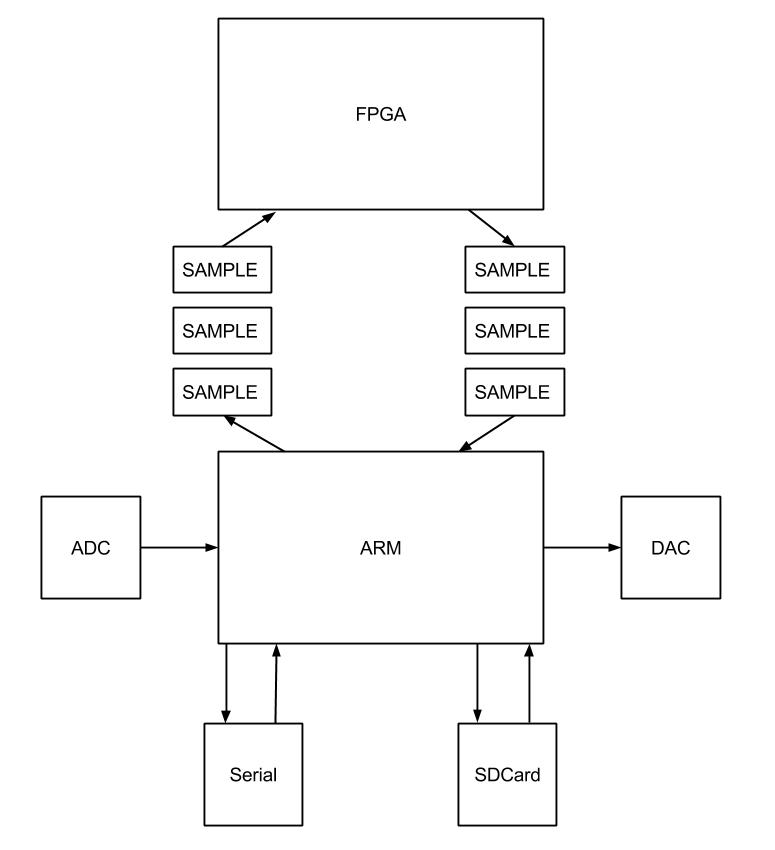
\includegraphics[height=150px]{figures/sw/sample-flow.png}
	%\begin{tikzpicture}[shorten >= 1pt, node distance=3cm, on grid, auto]
	%	\node[draw,rectangle,minimum size=2cm] (fpga) {FPGA};
	%	\node[draw,rectangle,below of=fpga,minimum size=2cm] (arm) {ARM};
	%\end{tikzpicture}
	\caption{Flow of samples}
	\label{fig:sw_sample_flow}
\end{figure}
\todo{Tikzify}


\subsection{External Bus Interface}
The MCU is connected to the FPGA and SRAM through the EBI. This leads to easy interfacing with these units as the EBI is memory mapped on the MCU. Communicating with the FPGA is done by reading and writing to memory. 

\todo{more about how the bus is implemented on the MCU}

\subsection{Direct Memory Access}
DMA provides the capability to move data without the intevention of the CPU. 
This is used extensively to implement the the dataflow in the low energy modes
that the MCU can run.

The core dataflow is from RAM on the MCU to the internal buffers on the FPGA 
and back to RAM on the MCU. 
\missingfigure{Figure showing RAM => FPGA => RAM}

In addition a DMA for each ADC and DAC are used when they are used as input and 
output respectively. When SDCard is used the contents of the files are read and
written by the CPU directly to and from RAM. 

\subsubsection{Deinterleaving of Samples}

Both when reading from a WAV file and from the ADC, samples from the
right and left channels are interleaved. The FPGA handles both channels in separat
pipelines. This is the reason for using two DMA channels

